\documentclass[12pt, a4paper]{ntut-report}
\usepackage[dvips,xetex]{graphicx}
\usepackage{ifpdf,mla}% <-- mla.sty requires ifpdf.sty, but (perversely) doesn't load it
%\usepackage{fontspec}
\usepackage{geometry}
\usepackage{lipsum}
\usepackage{xeCJK}
\usepackage{wallpaper}
\usepackage{pdfpages}
\usepackage{indentfirst}
\usepackage{setspace}
\usepackage{hyperref}
\usepackage{zhnumber}
\usepackage{titlesec}
\usepackage{amsmath}
\usepackage[backend=bibtex,sorting=none]{biblatex}
\usepackage{tabularx}
\usepackage{csquotes}
\usepackage{subcaption}

\MakeAutoQuote{“}{”}
\MakeOuterQuote{"}

\captionsetup{justification=centering,singlelinecheck=false,font={normalsize,stretch=2},labelsep=space}
\captionsetup[sub]{justification=centering,singlelinecheck=false,font={normalsize,stretch=2}}

\renewcommand{\baselinestretch}{1.5}
\xeCJKsetup{AutoFakeBold=true, AutoFakeSlant=true}
\setCJKmainfont{DFKai-SB.ttf} % 中文字體
\setmainfont{Times New Roman} % 英文字體
\geometry{a4paper,total={297mm,210mm},top=4.5cm,bottom=0.75cm,left=2.5cm,right=2.5cm} % 頁面設定，不需修改
\pagestyle{plain} % 頁碼
\addbibresource{reference.bib}

\input{ntut-labels.tex}

% 章節標題改為英文格式（Chapter 1, Chapter 2, ...）
\renewcommand\prechaptername{Chapter }
\renewcommand\postchaptername{}
\renewcommand\tocprechaptername{Chapter }
\renewcommand\tocpostchaptername{}
\renewcommand\countermapping[1]{\thechapter}

% 目錄、圖目錄、表目錄標題改為英文
\renewcommand\contentsname{Table of Contents}
\renewcommand\listfigurename{List of Figures}
\renewcommand\listtablename{List of Tables}

% 圖表標號改為英文
\renewcommand{\figurename}{Figure}
\renewcommand{\tablename}{Table}

\begin{document}

% 新增浮水印 Add Watermarks
\CenterWallPaper{.64}{ntut-logo.png}

% 封面（帶浮水印）Cover with a watermark
\input{page/titlepage.tex}
% 「學位論文口試委員會審定書」掃描檔，請檢附完整簽名之審定書掃描檔
% Please add "Oral Defense Committee Signature Form" with complete signatures.
\includepdf[pages=-]{static-page/signpage.pdf}

\pagenumbering{roman}

% 摘要頁（中文）Abstract (Chinese)
% If you don’t have Chinese abstract, please delete this one.
% 中文摘要頁
\begin{ZhAbstract}
    \begin{ZhAbstractItems}
        % 關鍵詞
        \noindent \text 關鍵詞：虛擬化、設備模擬、VirtIO、PCI transport

    \end{ZhAbstractItems}

    \begin{ZhAbstractDescription}
        輕量虛擬機器透過最小化映像檔來降低資源佔用與攻擊面，但同時移除了除錯與監控等工具。vmsh 針對此問題提出非合作式（non-cooperative）的解決方案，能在不修改虛擬機器監視器（hypervisor）與客體作業系統（Guest OS）的前提下，將 VirtIO 設備動態掛載至運行中的虛擬機器，為其補充所需的服務與工具。然而，vmsh 與 Cloud Hypervisor 在中斷機制上存在不相容，限制了 vmsh 的 hypervisor 支援範圍。

        本研究擴充 vmsh 的功能，在維持非合作式與 hypervisor 無關（hypervisor-agnostic）的特性前提下，為 vmsh 實現了 VirtIO over PCI transport，並利用 KVM 所提供的 KVM\_SIGNAL\_MSI 介面實現 MSI-X 中斷的注入，來解決 vmsh 在中斷機制上與 Cloud Hypervisor 的不相容問題。在 PCI 設備模擬方面，本研究延伸 vmsh 的 side-load library 機制在客體作業系統內部觸發 PCI rescan，並透過 ptrace 攔截客體作業系統發出的 Port I/O 指令，使其得以發現由 vmsh 所模擬的 PCI 虛擬設備，進而透過標準 virtio-pci 驅動程式與該設備進行 I/O 操作。

        此外，本研究在 QEMU 與 Cloud Hypervisor 兩種環境下完成功能驗證，並使用 xfstests 確認本研究中 PCI transport 實現的初步正確性，使 vmsh 成功支援 Cloud Hypervisor，擴展了 vmsh 的 hypervisor 支援範圍，並驗證了使用非合作式方法模擬 PCI 設備的可行性。
    \end{ZhAbstractDescription}

\end{ZhAbstract}

% 摘要頁（英文）Abstract (English)
% 英文摘要頁
\begin{EnAbstract}
    \begin{EnAbstractItems}
        % Keywords
        \noindent \text Keywords: Virtualization, Device Emulation, VirtIO, PCI Transport

    \end{EnAbstractItems}

    \begin{EnAbstractDescription}
        Lightweight virtual machines reduce resource consumption and attack surface by minimizing their images, but at the cost of removing debugging and monitoring tools. vmsh addresses this problem with a non-cooperative approach that dynamically attaches VirtIO devices to running virtual machines without modifying the hypervisor or the guest OS, supplementing VMs with the required services and tools. However, vmsh is incompatible with Cloud Hypervisor due to differences in interrupt mechanisms, limiting the range of hypervisors that vmsh can support.

        This study extends vmsh's functionality by implementing VirtIO over PCI transport while preserving its non-cooperative and hypervisor-agnostic properties. This study leverages the KVM\_SIGNAL\_MSI system call interface provided by KVM to inject MSI-X interrupts, resolving the interrupt mechanism incompatibility between vmsh and Cloud Hypervisor. For PCI device emulation, this study extends vmsh's side-load library mechanism to trigger PCI rescan within the guest OS, and intercepts Port I/O instructions issued by the guest via ptrace, enabling the guest OS to discover the PCI virtual device emulated by vmsh and perform I/O operations through the standard virtio-pci driver.

        Furthermore, this study conducts functional verification under both QEMU and Cloud Hypervisor environments, and uses xfstests to confirm the preliminary correctness of the PCI transport implementation. As a result, vmsh successfully supports Cloud Hypervisor, expanding its hypervisor compatibility and demonstrating the feasibility of emulating PCI devices using a non-cooperative approach.
    \end{EnAbstractDescription}

\end{EnAbstract}

% 鳴謝 Acknowledgements
\include{page/thanks.tex}
% 目錄、表目錄與圖目錄 Table of Contents, List of tables, List of figures
\include{page/table-of-content.tex}
 
\pagenumbering{arabic}

% 章節一 Chapter 1
\begin{ZhChapter}

\chapter{Introduction}
\label{ch:introduction}

\section{Background}
\label{sec:background}

Virtualization is a cornerstone of modern cloud computing. Cloud service providers consolidate multiple tenants onto a single physical host through virtual machines (VMs) to achieve resource sharing and isolation. Among the various virtualization solutions, KVM (Kernel-based Virtual Machine) in the Linux kernel leverages hardware-assisted virtualization to provide efficient full virtualization capabilities and has become the dominant virtualization API in the industry, widely adopted by major cloud providers.

As the demand for performance-sensitive workloads grows, the industry has seen a trend toward designing lightweight VMs. These approaches reduce the VM image size to lower memory footprint and accelerate startup time, making them suitable for rapid-deployment scenarios such as serverless computing, while also improving system reliability and security by reducing the attack surface. The key to achieving this lightweight design lies in minimizing the VM's root filesystem, which entails removing services that are not needed during normal operation, such as monitoring and debugging tools.

However, this lightweight strategy introduces a fundamental tension: when users need to debug, monitor, or attach additional services to a VM, these tools no longer exist in the VM image. Rebuilding the image is not only cumbersome but also requires restarting the VM, causing the loss of runtime state and diagnostic information. This trade-off between the advantages of lightweight VMs and the availability of functionality raises a central question: is it possible to dynamically extend the capabilities of a running VM without modifying its image?

To address this problem, Thalheim et al. proposed vmsh~\cite{Thalheim2022} at EuroSys 2022, a hypervisor-agnostic mechanism for extending VM functionality. The core idea of vmsh is to dynamically attach VirtIO devices to a running VM from the outside, without modifying the hypervisor's source code or altering the guest image. Specifically, vmsh traces the hypervisor process using Linux's ptrace mechanism and leverages the KVM interface to side-load code into the guest kernel, registering VirtIO block and console devices within the guest to provide capabilities such as filesystem mounting and interactive terminal access. At the device emulation level, vmsh employs VirtIO MMIO transport as the communication channel between host and guest, and uses KVM's irqfd mechanism for interrupt injection. This approach has been successfully validated on multiple mainstream KVM hypervisors, including QEMU, Firecracker, crosvm, and kvmtool, demonstrating its cross-hypervisor generality.

\section{Motivations}
\label{sec:motivations}

Despite vmsh's demonstrated cross-hypervisor generality, a gap remains in its actual support coverage. Among the five KVM hypervisors it targets, Cloud Hypervisor, initiated by Intel, is the sole exception that remains incompatible. The authors of vmsh explicitly noted in their paper:

\begin{quote}
\textit{VMSH is able to support 4 out of the 5 hypervisors. Cloud Hypervisor is the exception as it uses PCIe's MSI-X messages for its interrupt handling. Therefore, it is incompatible with MMIO as a VirtIO transport channel.}~\cite{Thalheim2022}
\end{quote}

vmsh's existing dynamic device attachment is implemented using VirtIO MMIO transport, whose interrupt injection relies on the interrupt routing mechanism internal to the KVM kernel. However, Cloud Hypervisor adopts a different interrupt architecture, rendering the interrupt path that vmsh depends on inoperable and consequently making the entire MMIO transport approach unusable on the Cloud Hypervisor platform.

To address this limitation, the authors of vmsh also outlined a research direction: ``We plan to extend VMSH to support VirtIO over PCI for Cloud Hypervisor.''~\cite{Thalheim2022} This implies that the virtual devices dynamically attached by vmsh would no longer be presented via MMIO transport but would instead appear as PCI devices within the guest OS, using MSI-X interrupt injection to replace the incompatible interrupt path and thereby resolving the compatibility issue with Cloud Hypervisor.

However, implementing VirtIO over PCI in a non-cooperative environment is fundamentally different from PCI device emulation performed internally by a hypervisor. In a typical virtualization architecture, PCI device emulation is handled within the hypervisor, which has full access to PCI bus topology information and can directly manage device registration, configuration space responses, and interrupt routing. By contrast, vmsh operates outside the hypervisor and cannot access these internal data structures and interfaces; it must achieve the same objectives through indirect means. Specifically, as an external process independent of the hypervisor, vmsh faces the following technical challenges: first, intercepting the guest's accesses to PCI configuration space to enable virtual device discovery and configuration; second, injecting MSI-X interrupts to replace the incompatible interrupt path; and third, implementing complete VirtIO-PCI device emulation, including the Capabilities structure, BAR mapping, and virtqueue management.

In summary, the design of vmsh pursues two core objectives: non-cooperativeness, requiring no pre-deployed programs in the guest userspace, and generality, not relying on the internal interfaces of any specific hypervisor. As discussed above, vmsh's existing MMIO transport approach cannot support Cloud Hypervisor, while implementing PCI device emulation from outside the hypervisor involves several unresolved technical challenges. Therefore, how to implement VirtIO over PCI transport while maintaining vmsh's non-cooperative and hypervisor-agnostic design philosophy, thereby enabling vmsh to support Cloud Hypervisor, is the central research question that this study aims to address.

\section{Research Contribution}
\label{sec:contribution}

This study extends vmsh to address its incompatibility with Cloud Hypervisor by implementing VirtIO over PCI transport in a non-cooperative environment. The main contributions are as follows:

\begin{sloppypar}
\textbf{Non-cooperative PCI device emulation.} As an external process independent of the hypervisor, vmsh must complete device emulation from the outside without hypervisor cooperation. This study extends vmsh's side-load library mechanism to trigger a PCI rescan within the guest OS and intercepts Port I/O instructions issued by the guest via ptrace, implementing PCI device discovery, configuration space emulation, BAR mapping, and VirtIO-PCI negotiation, enabling the guest to access the device emulated by vmsh through the standard virtio-pci driver.
\end{sloppypar}

\begin{sloppypar}
\textbf{Resolving interrupt mechanism compatibility and extending hypervisor support.} vmsh's existing interrupt injection mechanism relies on the Full IRQChip architecture and cannot operate under Cloud Hypervisor's Split IRQChip environment. This study adopts the KVM\_SIGNAL\_MSI interface provided by KVM to implement MSI-X interrupt injection, making the interrupt mechanism independent of IRQChip architecture differences.
\end{sloppypar}

\begin{sloppypar}
\textbf{Cross-hypervisor validation of correctness and generality.} Functional validation is performed under both QEMU and Cloud Hypervisor environments to confirm the generality of PCI transport; additionally, correctness testing using xfstests is conducted under the QEMU environment to confirm the preliminary correctness of PCI transport.
\end{sloppypar}

\section{Thesis Organization}
\label{sec:organization}

\textbf{Chapter~\ref{ch:introduction} Introduction} presents the background and motivation of this study, describes the incompatibility between vmsh and Cloud Hypervisor, and states the contributions of this research.

\textbf{Chapter~\ref{ch:literature} Literature Review} reviews the technical background relevant to this study, including the KVM virtualization architecture, the VirtIO device model, the PCI bus and MSI-X interrupt mechanism, and introduces the system architecture and design of vmsh.

\textbf{Chapter~\ref{ch:method} Proposed Method} details the system design and implementation of this study, covering PCI device discovery, Port I/O interception, VirtIO-PCI device emulation, and MSI-X interrupt injection.

\textbf{Chapter~\ref{ch:experiment} Experiment and Result} presents the validation results of this study, including functional validation under QEMU and Cloud Hypervisor, correctness testing with xfstests, and a discussion of the limitations of the prototype implementation.

\textbf{Chapter~\ref{ch:conclusion} Conclusion and Future Work} summarizes the results and contributions of this study, and proposes future research directions including an asynchronous I/O model, performance testing, and integration with vmsh's broader functionality.

\end{ZhChapter}

% 章節二 Chapter 2
\begin{ZhChapter}

\chapter{若標題太長，則可以分成兩行排列的形式撰寫}

\section{名詞定義（小標）}

定義定義定義定義定義定義\cite{latex2e}，定義定義定義定義，定義定義定義定義定義定義定義定義定義定義，定義定義。

\begin{table*}[htbp]
    \centering
    \caption{表格範例標題} \label{tab: complexity}
    \makebox[\linewidth][c]{
    \renewcommand\arraystretch{1.2}{
        \begin{tabular}{| l | c  c  c  c |}
        \hline
        Protocol & $P$ & $CS_1$ & $CS_2$ & $RG$ \\
        \hline
        MSSMul & $O(1)$, $O(1)$, N/A & $O(n-t)$, $O(n)$, $O(1)$ & $O(n-t)$, $O(n)$, N/A & $O(1)$, $O(n)$, $O(n)$ \\
        SC & $O(1)$, $O(1)$, N/A & $O(n-t)$, $O(n)$, $O(1)$ & $O(n-t)$, $O(n)$, N/A & $O(1)$, $O(n)$, $O(n)$ \\
        \hline 
        \end {tabular}
    }}
\end {table*}

\section{模型說明（小標）}

說明說明說明說明，說明說明說明說明說明說明說明說明說明說明說明說明，說明說明說明說明說明說明說明說明。

\begin{figure*}[htbp]
    \centering
    \includegraphics[width = 0.5\textwidth]{image.jpeg}
    \caption{Cool train station}
    \label{fig: image}
\end{figure*}

% ===== 以下為轉換演示 =====

\section{VMSH: Hypervisor-agnostic Guest Overlays for VMs}

\subsection{System Architecture}

As an independent host process, vmsh runs alongside the hypervisor on the same host machine. vmsh does not modify the hypervisor's source code, nor does it rely on any management API provided by the hypervisor. Instead, vmsh completes all operations externally through ptrace and the underlying KVM API. Figure~\ref{fig:vmsh-arch} presents the system architecture of vmsh (adapted from \cite{Thalheim2022} Figure 2), whose workflow can be divided into the following four steps:

\begin{figure*}[htbp]
    \centering
    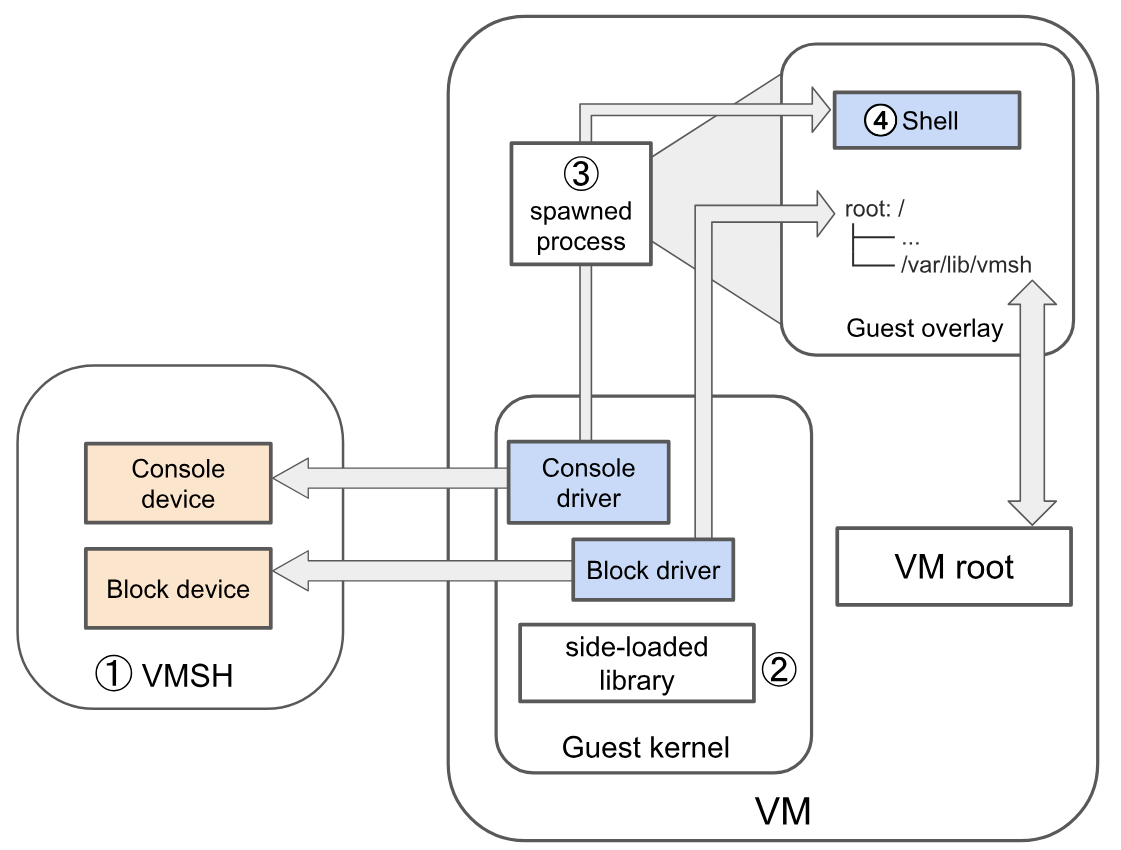
\includegraphics[width=0.8\textwidth]{figures/vmsh-arch.png}
    \caption{System architecture of vmsh. vmsh establishes devices in the guest through side-loading a kernel library. The block device supports the overlay root file system, and the console device handles the I/O of the spawned process. Numbers 1--4 correspond to the four-step workflow. (Adapted from \cite{Thalheim2022})}
    \label{fig:vmsh-arch}
\end{figure*}

% ===== 演示結束 =====

\end{ZhChapter}
% 章節三 Chapter 3
\begin{ZhChapter}

\chapter{Proposed Method}
\label{ch:method}

\section{System Architecture Overview}
\label{sec:arch-overview}

The device emulation of the original vmsh~\cite{Thalheim2022} is built upon the VirtIO MMIO transport. As shown in Figure~\ref{fig:vmsh-mmio-arch}, vmsh operates as an independent host process external to the hypervisor, using ptrace to trace the hypervisor process for device emulation and control. When the VirtIO driver within the guest accesses device registers in the MMIO region, a KVM\_EXIT\_MMIO VM-Exit is triggered, which vmsh intercepts via ptrace and handles the device-side response. For interrupt injection, vmsh uses KVM's irqfd mechanism: when the device needs to notify the guest, vmsh writes to an eventfd, and upon receiving the event, KVM routes the interrupt through the GSI routing table to the in-kernel IOAPIC, which then delivers it to the target vCPU. The in-kernel IOAPIC and GSI routing table are established by the hypervisor during startup via KVM\_CREATE\_IRQCHIP and KVM\_SET\_GSI\_ROUTING; vmsh itself does not participate in building this infrastructure but rather directly uses and depends on its existence within the interrupt path.

\begin{figure*}[htbp]
    \centering
    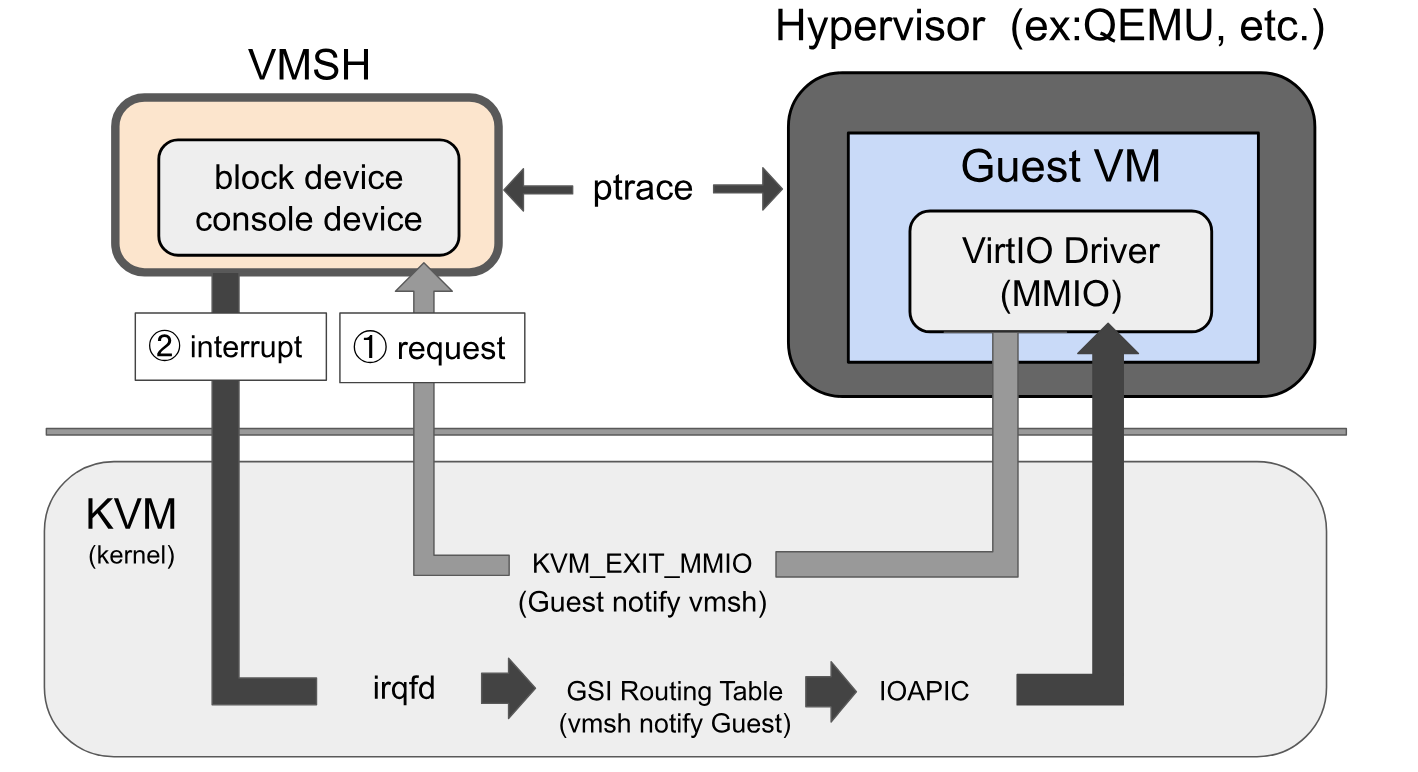
\includegraphics[width=1.0\textwidth]{figures/vmsh-mmio-arch.png}
    \caption{vmsh Original Architecture (VirtIO-MMIO Transport)}
    \label{fig:vmsh-mmio-arch}
\end{figure*}

In Figure~\ref{fig:vmsh-mmio-arch}, (1) indicates the guest notifying vmsh to process I/O requests through the MMIO region, and (2) indicates vmsh delivering interrupts to the guest via irqfd through the GSI Routing Table and in-kernel IOAPIC. The path of (2) depends on the interrupt routing infrastructure established by the hypervisor, which does not exist on Cloud Hypervisor.

The above architecture works correctly on QEMU, Firecracker, crosvm, and kvmtool, as these hypervisors all adopt the Full IRQChip mode, where the KVM kernel internally manages the complete interrupt routing infrastructure, which is compatible with vmsh's existing implementation. However, Cloud Hypervisor adopts the Split IRQChip architecture, where the IOAPIC is implemented by Cloud Hypervisor in userspace; the KVM kernel contains no in-kernel IOAPIC and no corresponding GSI routing table. This means that the irqfd interrupt path on which vmsh's existing implementation depends does not exist on Cloud Hypervisor; after writing to the eventfd, the interrupt signal cannot be delivered to the guest due to the absence of the corresponding routing infrastructure. This renders vmsh's existing MMIO transport approach inapplicable on Cloud Hypervisor.

\begin{figure*}[htbp]
    \centering
    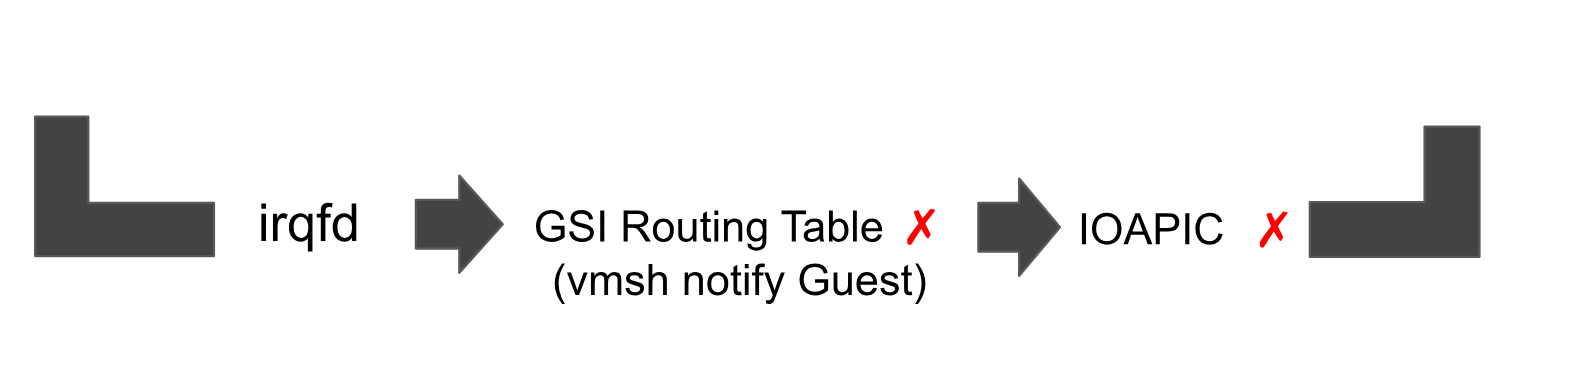
\includegraphics[width=0.8\textwidth]{figures/irqfd-broken.png}
    \caption{vmsh's Existing irqfd Interrupt Path Unavailable on Cloud Hypervisor (Split IRQChip)}
    \label{fig:irqfd-broken}
\end{figure*}

\begin{sloppypar}
To resolve the above incompatibility, an interrupt mechanism that does not depend on GSI routing or the IOAPIC is needed. This study uses the KVM\_SIGNAL\_MSI~\cite{KVMAPI} ioctl to write interrupt messages directly to the vCPU's Local APIC, bypassing the GSI routing table and IOAPIC, thus working regardless of whether the hypervisor adopts a Full or Split IRQChip architecture.
\end{sloppypar}

\begin{sloppypar}
KVM\_SIGNAL\_MSI is a KVM ioctl for sending MSI-X type interrupts, requiring the address and data of the interrupt vector in MSI-X format. MSI-X is an interrupt mechanism specific to PCI devices, with interrupt vectors stored in the PCI device's MSI-X Table; only PCI devices possess this structure. Therefore, adopting KVM\_SIGNAL\_MSI necessarily requires the device to support MSI-X interrupts, which in turn means implementing, beyond the existing MMIO transport, a complete VirtIO-PCI transport for vmsh, enabling the guest to discover and access vmsh's virtual device through standard PCI mechanisms and receive MSI-X type interrupt notifications.
\end{sloppypar}

Based on the above analysis, this study proposes \textbf{Non-cooperative PCI Device Emulation}, introducing PCI transport to vmsh to resolve the interrupt path unavailability issue. Figure~\ref{fig:vmsh-pci-arch} shows the PCI transport architecture implemented in this study, contrasting with the MMIO transport in Figure~\ref{fig:vmsh-mmio-arch}. In Figure~\ref{fig:vmsh-pci-arch}, (1) indicates the guest accessing PCI configuration space (0xCF8/0xCFC) via KVM\_EXIT\_IO and accessing BAR regions via KVM\_EXIT\_MMIO, both intercepted and handled by vmsh. (2) indicates vmsh delivering interrupts to the guest by writing directly to the LAPIC via KVM\_SIGNAL\_MSI, without depending on the GSI Routing Table and IOAPIC. Stage1 is responsible for triggering PCI rescan during VM runtime, enabling the guest to discover and initialize the virtual device. Items marked with a star ($\star$) in the figure indicate components added by this study.

\begin{figure*}[htbp]
    \centering
    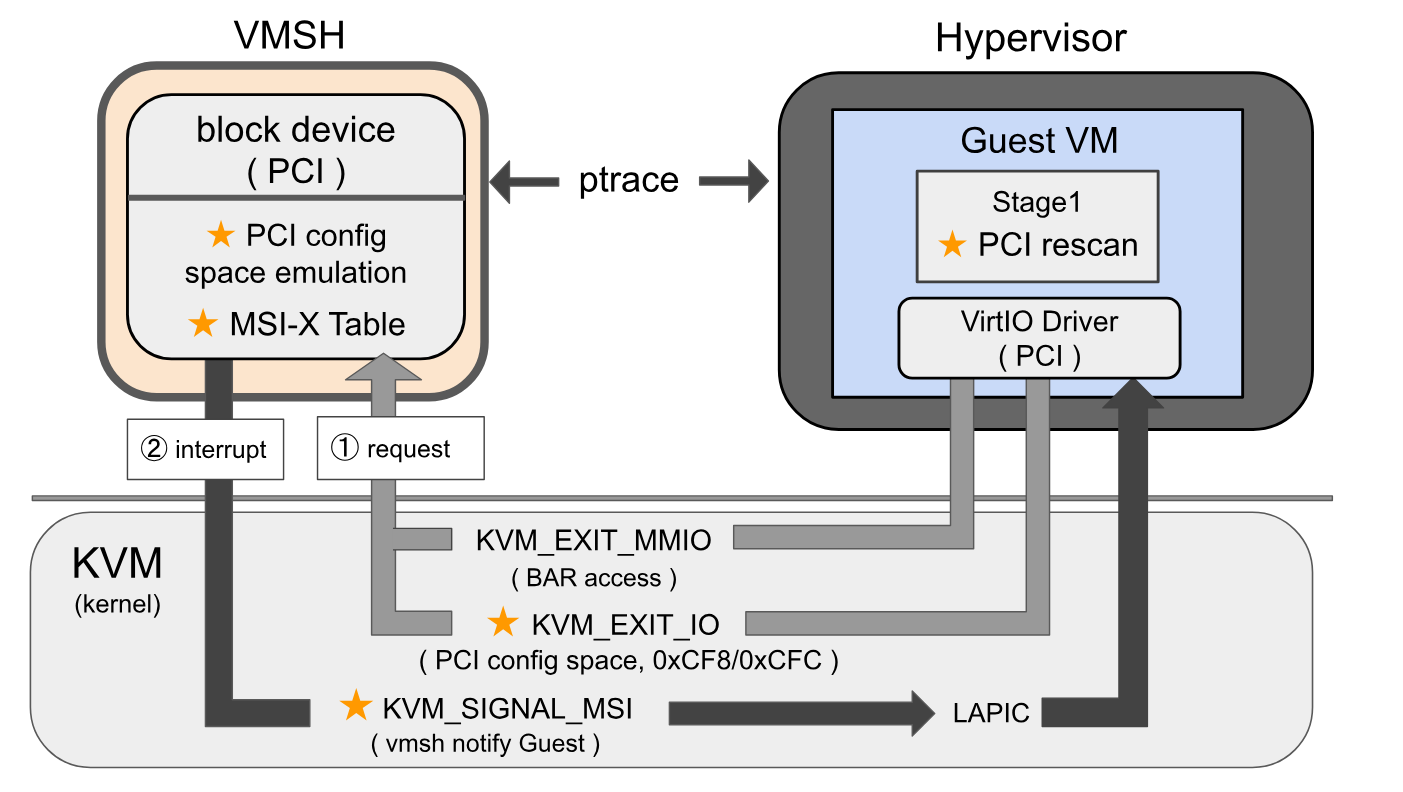
\includegraphics[width=1.0\textwidth]{figures/vmsh-pci-arch.png}
    \caption{System Architecture (PCI Transport). Stars ($\star$) Indicate Components Added by This Study.}
    \label{fig:vmsh-pci-arch}
\end{figure*}

As an extension of vmsh, the design of this study follows vmsh's two core principles:

\begin{itemize}
    \item \textbf{Non-cooperativeness}: No reliance on programs pre-installed in the guest OS for cooperative operation.
    \item \textbf{Generality}: No dependence on any specific hypervisor's API; the design is not tied to any particular hypervisor's mechanisms and supports a wide range of guest kernel versions.
\end{itemize}

To implement PCI transport under these constraints, this study's design references and extends vmsh's existing implementation mechanisms, including its ptrace-based I/O interception framework and Stage1 injection mechanism, so that the PCI transport implementation extends vmsh's compatibility while maintaining vmsh's original non-cooperative and hypervisor-agnostic characteristics. The design goal of this study is to enable vmsh to perform device emulation through PCI transport and to be applicable to multiple KVM-based hypervisors.

As an independent process running alongside the hypervisor, vmsh's device emulation must be completed externally without hypervisor cooperation. Therefore, to implement non-cooperative PCI device emulation, the following core problems need to be addressed:

\textbf{1. Device discovery.} vmsh attaches devices dynamically during VM runtime, thus requiring a mechanism for the guest to discover newly attached virtual devices. This study extends vmsh's side-load library mechanism, leveraging its ability to load and execute code within the guest kernel to trigger PCI rescan, giving vmsh the capability to trigger PCI device initialization in the guest from outside the hypervisor (Section~\ref{sec:pci-rescan}).

\textbf{2. Port I/O interception.} During PCI device initialization, the guest accesses the PCI configuration space through Port I/O instructions to interact with the virtual device. Since vmsh's existing implementation only has the capability to intercept MMIO type I/O accesses, and the hypervisor also processes these Port I/O accesses, vmsh's interception must avoid mutual interference with the hypervisor. This study applies concepts similar to vmsh's existing MMIO interception techniques to Port I/O interception, implementing and validating vmsh's ability to intercept and handle Port I/O accesses (Section~\ref{sec:port-io}).

\textbf{3. PCI device emulation.} After the guest discovers the device, it needs to complete initialization and perform I/O data exchange with the device through the standard VirtIO-PCI protocol. vmsh's existing implementation only supports VirtIO-MMIO devices; this study implements VirtIO-PCI device emulation, including PCI configuration space, Capabilities structure, BAR mapping, and virtqueue setup, enabling the guest to communicate with the device emulated by vmsh through the standard VirtIO-PCI driver (Section~\ref{sec:virtio-pci-emulation}).

\begin{sloppypar}
\textbf{4. Interrupt notification.} After processing an I/O request, the device needs to notify the guest. As described above, vmsh's existing irqfd interrupt path is unavailable on Cloud Hypervisor; this study maintains the interrupt vectors written by the guest driver to the virtual PCI device's MSI-X Table and uses KVM\_SIGNAL\_MSI to deliver interrupts directly to the LAPIC, implementing a notification mechanism distinct from vmsh's existing interrupt path (Section~\ref{sec:msix-injection}).
\end{sloppypar}

\textbf{5. I/O data path.} To verify the feasibility and correctness of the above mechanisms, this study adopts a synchronous I/O model as a prototype, integrating device discovery, Port I/O interception, PCI device emulation, and interrupt notification to implement a complete data path from the guest issuing an I/O request to receiving an MSI-X interrupt response.

In summary, this study resolves the interrupt path incompatibility issue of vmsh on Cloud Hypervisor by introducing PCI transport, and implements a complete non-cooperative PCI device emulation scheme covering device discovery, Port I/O interception, PCI device emulation, and interrupt notification, while maintaining vmsh's original design philosophy. The following sections elaborate on each mechanism designed in this study, in the order of the device lifecycle.

\section{PCI Bus Rescan and Device Discovery}
\label{sec:pci-rescan}

vmsh needs to attach devices dynamically during VM runtime; however, the guest kernel has already completed PCI bus scanning during the boot phase and does not proactively rescan the PCI bus at runtime. Therefore, vmsh requires a mechanism that allows the guest to discover vmsh's PCI virtual device during VM runtime. This study extends and applies vmsh's Stage1 mechanism, using Stage1 to trigger the guest kernel to rescan the PCI bus, enabling the guest to detect newly attached virtual devices at runtime. The following describes how PCI rescan is triggered, and how the guest kernel discovers and initializes the virtual device injected by vmsh during the rescan process.

\subsection{PCI Rescan Trigger Mechanism}
\label{sec:rescan-trigger}

\begin{sloppypar}
During VM boot, the guest kernel performs a full PCI bus scan, enumerating all Bus/Device/Function (BDF) slots and registering discovered devices with the system. This scan occurs before vmsh attach, so vmsh cannot insert virtual devices during the boot scan and requires a method to make the guest kernel rescan the PCI bus during VM runtime.
\end{sloppypar}

The Linux kernel provides the \texttt{/sys/bus/pci/rescan} interface; writing \texttt{1} to this file triggers a PCI bus rescan. This study extends vmsh's side-load library mechanism to utilize this interface: vmsh loads and executes code within the guest kernel through Stage1 (see Section~\ref{sec:vmsh}), and this study implements a \texttt{trigger\_pci\_rescan()} function in Stage1 that opens \texttt{/sys/bus/pci/rescan} and writes \texttt{1} within the guest kernel context, triggering the guest kernel to rescan the PCI bus. Since Stage1 runs in guest kernel mode and has permission to access sysfs, it can directly operate this interface.

The key aspect of this method is that rescan differs in behavior from the cold boot scan. The cold boot scan enumerates all BDF slots, whereas rescan skips devices already registered in the system and only scans BDF slots that are not yet occupied. Figure~\ref{fig:pci-rescan-code} shows the simplified PCI rescan logic in the Linux kernel.

\begin{figure*}[htbp]
    \centering
    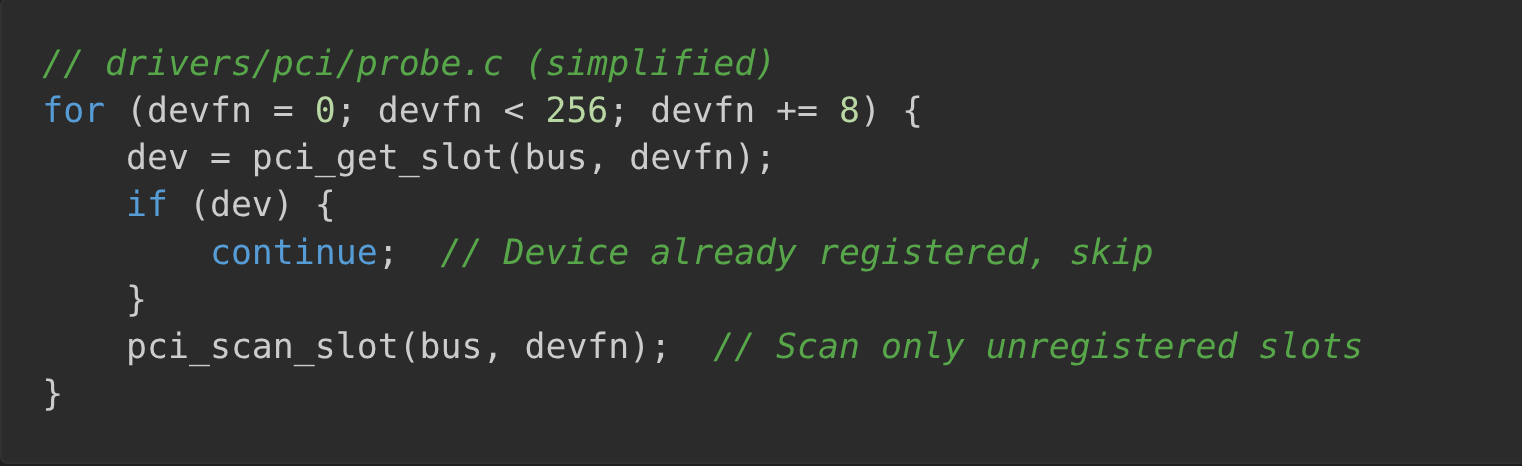
\includegraphics[width=0.95\textwidth]{figures/pci-rescan-code.png}
    \caption{Simplified PCI Rescan Logic in the Linux Kernel (drivers/pci/probe.c)}
    \label{fig:pci-rescan-code}
\end{figure*}

This behavior means that the rescan triggered by vmsh does not interfere with PCI devices already established by the hypervisor in the VM. For example, in a QEMU environment, devices created by the hypervisor such as VirtIO Block, VirtIO RNG, and ISA Bridge are already registered during boot; rescan skips these registered BDF slots and only probes empty ones. Therefore, rescan is safe and does not affect normal VM operation.

\subsection{Rescan Process and Virtual Device Discovery}
\label{sec:rescan-discovery}

\begin{sloppypar}
During rescan, the guest kernel reads the Vendor ID (configuration space offset 0x00) of each unregistered BDF slot through the PCI configuration space access mechanism (0xCF8/0xCFC I/O ports). If the Vendor ID is 0xFFFF or 0x0000, the guest kernel determines that no device exists at that slot and skips it; if the value is valid, the guest kernel considers a device present and proceeds to read the full configuration space for device initialization.
\end{sloppypar}

vmsh selects in advance a BDF slot not used by the hypervisor as the address of the virtual device. When the guest kernel scans that slot during rescan, vmsh responds with a valid Vendor ID and Device ID through I/O interception techniques (detailed in Section~\ref{sec:port-io}), causing the guest kernel to recognize a device at that slot. For other empty slots, vmsh does not intervene, and the guest kernel receives 0xFFFF from the hypervisor and skips them normally.

Figure~\ref{fig:pci-rescan-example} illustrates this process using a QEMU environment as an example, assuming vmsh has selected BDF 00:0a.0 as the virtual device's slot.

\begin{figure*}[htbp]
    \centering
    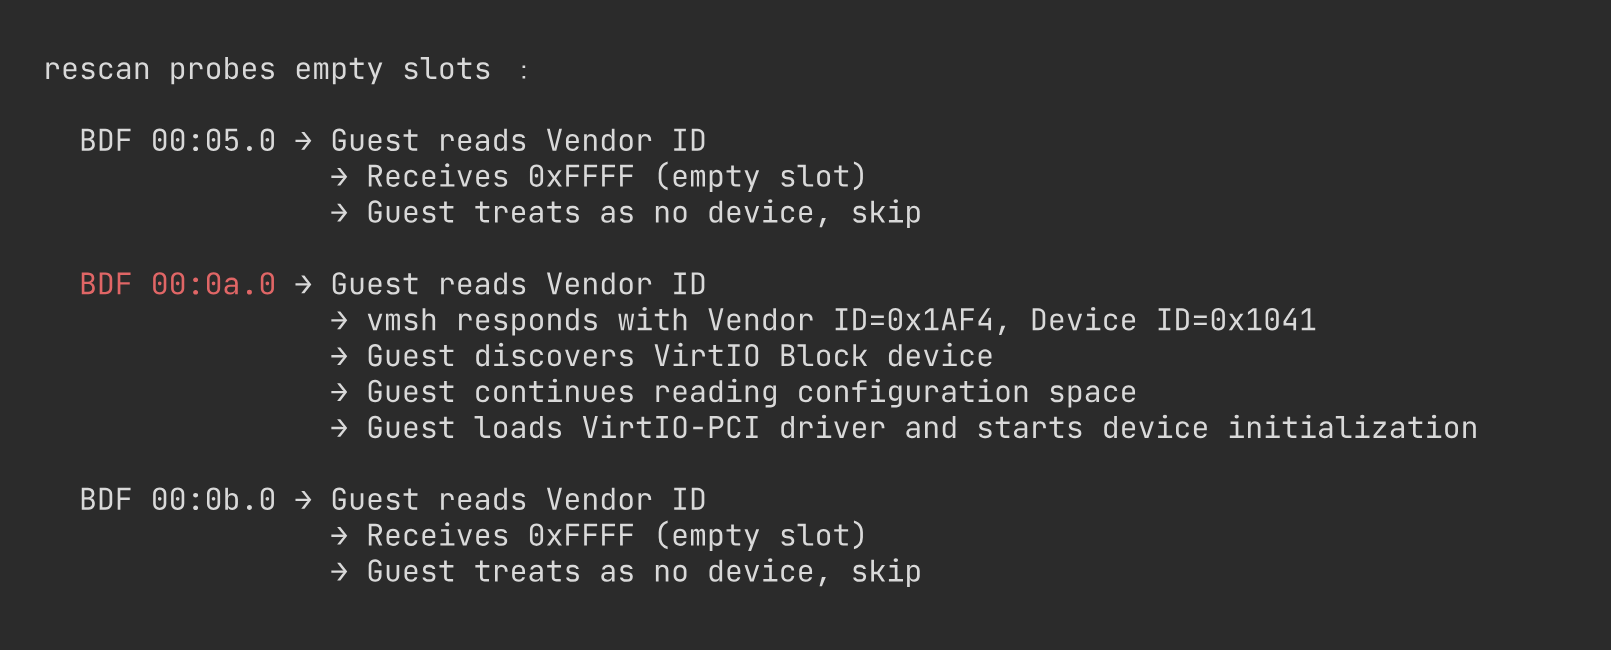
\includegraphics[width=1.0\textwidth]{figures/pci-rescan-example.png}
    \caption{PCI Rescan Behavior with a vmsh Virtual PCI Device at BDF 00:0a.0}
    \label{fig:pci-rescan-example}
\end{figure*}

Upon receiving a valid Vendor ID, the guest kernel determines that a device exists at the BDF slot and proceeds with the subsequent PCI device initialization process, including reading the full configuration space and allocating system resources required by the device. The specific details of this initialization process are described in Section~\ref{sec:virtio-pci-emulation}.

\section{Port I/O Interception Mechanism}
\label{sec:port-io}

Section~\ref{sec:pci-rescan} described how vmsh triggers PCI rescan to allow the guest to discover virtual devices. During the rescan process, the guest interacts with devices through the PCI configuration space access mechanism (0xCF8/0xCFC I/O ports), and vmsh needs to intercept these I/O accesses and respond with the virtual device's configuration data. This section first describes the two types of I/O exits in KVM, then explains how this study implements Port I/O interception and handling logic for vmsh, and finally describes how to prevent the hypervisor from overwriting vmsh's responses.

\subsection{Two Types of I/O Exits}
\label{sec:io-exit-types}

When the guest performs I/O operations, KVM generates a VM-Exit and records the relevant information in the kvm\_run shared memory structure for the hypervisor to read and process. Depending on the I/O access method, KVM distinguishes between two exit types:

\begin{itemize}
    \item \textbf{KVM\_EXIT\_MMIO}: Triggered when the guest accesses an unmapped memory address. The kvm\_run structure records the physical address (phys\_addr), data length (len), data content (data), and read/write direction (is\_write). Device register accesses for VirtIO MMIO transport belong to this type.

    \item \textbf{KVM\_EXIT\_IO}: Triggered when the guest executes Port I/O instructions (IN/OUT). The kvm\_run structure records the I/O port address (port), access direction (direction, distinguishing IN and OUT), data length (size), and the offset of the data within the kvm\_run structure (data\_offset). PCI configuration space accesses (0xCF8/0xCFC) belong to this type.
\end{itemize}

vmsh's existing implementation already has the ability to intercept KVM\_EXIT\_MMIO, used for handling device register accesses of VirtIO MMIO transport. However, PCI configuration space accesses are performed through Port I/O, which triggers KVM\_EXIT\_IO, and vmsh did not originally have the ability to intercept this type of event. To implement PCI transport, this study adds KVM\_EXIT\_IO interception and handling mechanisms to vmsh.

\subsection{Port I/O Interception Handling}
\label{sec:port-io-handling}

\begin{sloppypar}
vmsh's I/O interception is built upon the ptrace mechanism. vmsh uses ptrace to trace the thread in the hypervisor process responsible for executing the vCPU; when the hypervisor calls \texttt{ioctl(KVM\_RUN)} to execute the vCPU and returns due to a VM-Exit, vmsh intercepts this event at the ptrace syscall-exit stop point. At this point, vmsh can read the kvm\_run structure from the hypervisor process's memory via ptrace to obtain the VM-Exit type and related information.
\end{sloppypar}

As described in Section~\ref{sec:pci-transport}, x86 PCI configuration space access is performed through two I/O ports: the guest first writes the target BDF address to 0xCF8 (CONFIG\_ADDRESS) using an \texttt{out} instruction, then reads or writes the configuration data at that location through 0xCFC (CONFIG\_DATA) using an \texttt{in} or \texttt{out} instruction. In a KVM environment, these two Port I/O operations each trigger a separate KVM\_EXIT\_IO event, with the direction field in the kvm\_run structure using IN and OUT to distinguish the type of instruction the guest executed.

\begin{sloppypar}
This study implements the following KVM\_EXIT\_IO handling logic for vmsh, divided into two phases based on port: when vmsh intercepts an event with port = 0xCF8 and direction = OUT, it reads the value written by the guest from the data\_offset location, parses the Bus/Device/Function and Register fields, and records the target BDF address the guest is currently accessing. When vmsh intercepts an event with port = 0xCFC, it checks whether the previously recorded BDF address corresponds to the virtual device's slot. If not, vmsh does not intervene and lets the hypervisor respond normally. If it is the virtual device, vmsh distinguishes between read and write based on direction: for direction = IN, vmsh writes the corresponding register value of the virtual device to the data\_offset location in the kvm\_run structure as the read response to the guest; for direction = OUT, vmsh reads the value written by the guest from the data\_offset location and updates the virtual device's internal state.
\end{sloppypar}

\subsection{Response Protection Mechanism}
\label{sec:response-protection}

The handling logic in Section~\ref{sec:port-io-handling} enables vmsh to respond with the virtual device's configuration data; however, vmsh and the hypervisor both process the same KVM\_EXIT\_IO event, and without protection, the hypervisor's subsequent processing would overwrite the response vmsh has already written. This section explains the cause of this problem and its solution.

Since 0xCF8/0xCFC are standard PCI configuration space I/O ports, the hypervisor itself also processes these Port I/O events. After vmsh releases control, the hypervisor continues to process the same KVM\_EXIT\_IO event. For IN-direction accesses, the hypervisor queries its own managed PCI devices, and since vmsh's virtual device does not exist in the hypervisor's device list, the hypervisor treats the slot as empty and responds with 0xFFFF, overwriting the data vmsh previously wrote.

\begin{sloppypar}
vmsh's existing MMIO interception has faced the same problem and solves it by modifying the direction field in the kvm\_run structure: when responding to a KVM\_EXIT\_MMIO read request, after vmsh writes data to the data field of kvm\_run, it changes \texttt{is\_write} from 0 to 1, causing the hypervisor to treat the event as a write operation and perform no substantive processing, thereby avoiding overwriting vmsh's response. This study applies the same concept to Port I/O interception: after writing the response data to data\_offset, vmsh changes the direction field in the kvm\_run structure from IN to OUT. When the hypervisor subsequently processes this event, it sees an OUT-direction access; for an OUT instruction writing to a nonexistent PCI slot, the hypervisor performs no operation (no-op), thus preserving the data vmsh has written. On the next VM-Entry, KVM loads the data at the data\_offset location into the guest's registers, allowing the guest to receive the virtual device configuration data responded by vmsh.
\end{sloppypar}

Figure~\ref{fig:direction-change} uses the example of the guest reading the virtual device's Vendor ID to contrast the behavior without and with the response protection mechanism. (a) If vmsh only writes the response data without modifying direction, the hypervisor overwrites vmsh's data with an empty slot response. (b) After vmsh changes direction from IN to OUT, the hypervisor's write to an empty slot produces no operation, and vmsh's response data is preserved.
\newpage

\begin{figure*}[htbp]
    \centering
    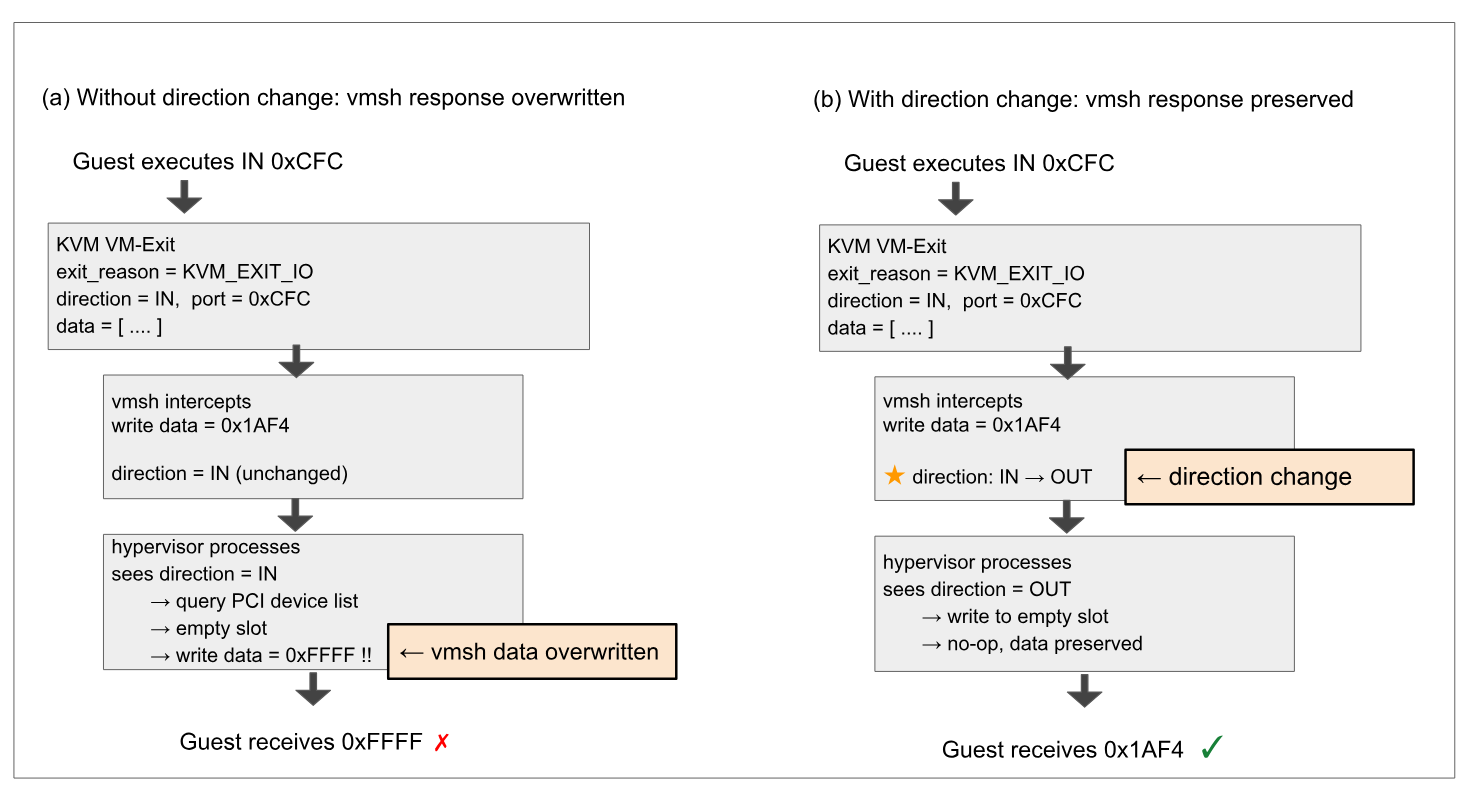
\includegraphics[width=1.0\textwidth]{figures/direction-change.png}
    \caption{Illustration of Response Protection Mechanism}
    \label{fig:direction-change}
\end{figure*}

This response protection mechanism shares the same core idea as vmsh's existing MMIO interception: by modifying the direction field in the kvm\_run structure, the hypervisor is prevented from performing substantive processing on the event, thereby avoiding overwriting the response data written by vmsh.

In summary, this study builds upon vmsh's existing ptrace infrastructure, specifically the ability to access the hypervisor's kvm\_run shared memory structure and intercept VM-Exit events via ptrace, and implements a Port I/O interception and handling mechanism on top of this foundation. Through this mechanism, vmsh is able to allow the guest to access the PCI device configuration space emulated by vmsh in a non-cooperative manner.

\section{VirtIO-PCI Device Emulation}
\label{sec:virtio-pci-emulation}

Section~\ref{sec:port-io} gave vmsh the ability to intercept the guest's PCI configuration space accesses. This section describes how vmsh emulates the VirtIO-PCI device's configuration space and connects to vmsh's existing MMIO interface, enabling the guest driver to communicate with vmsh and complete the PCI device initialization process.

\subsection{Initialization Process Overview}
\label{sec:init-overview}

\begin{figure*}[htbp]
    \centering
    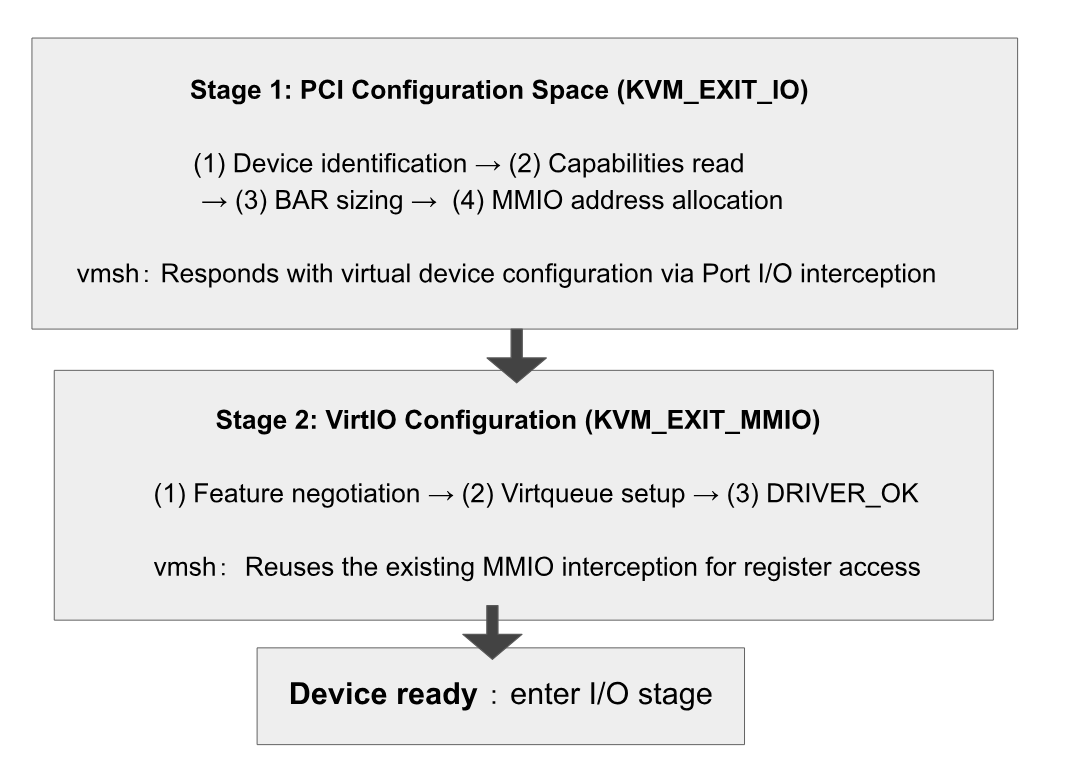
\includegraphics[width=0.9\textwidth]{figures/pci-init-stages.png}
    \caption{Two Stages of VirtIO-PCI Device Initialization}
    \label{fig:pci-init-stages}
\end{figure*}

From discovery by the guest to becoming ready for I/O, a VirtIO-PCI device goes through two initialization stages, each using a different access mechanism:

The first stage is completed through the PCI configuration space, using the Port I/O interception mechanism described above. The guest driver reads the device's basic information (Vendor ID, Device ID, Class Code, etc.) through the configuration space, then traverses the Capabilities linked list to identify the functions supported by the device and the BAR locations corresponding to each functional region. The PCI subsystem then probes the size of each BAR through the BAR sizing mechanism and allocates MMIO addresses for them. All accesses in this stage are performed through 0xCF8/0xCFC I/O ports, triggering KVM\_EXIT\_IO, which vmsh intercepts and responds with the virtual device's configuration data.

The second stage is performed through the BAR MMIO addresses allocated in the first stage. The guest driver accesses the registers of each functional region based on the BAR and offset information recorded in the Capabilities, completing the VirtIO handshake with vmsh: negotiating mutually supported features, setting up the virtqueue descriptor table and ring buffer addresses, and finally writing the DRIVER\_OK flag to mark the device as ready. Accesses in this stage trigger KVM\_EXIT\_MMIO, which is handled by vmsh's existing MMIO interception mechanism.

After both stages are complete, the device enters the I/O processing phase.

\subsection{PCI Configuration Space Stage}
\label{sec:config-space-stage}

During the first stage of initialization, the guest driver interacts with the virtual device through the PCI configuration space, and vmsh needs to respond with correct configuration data for each read. This study implements a complete VirtIO-PCI configuration space for vmsh, covering three parts: device identification, Capabilities linked list, and BAR sizing.

\noindent\textbf{Device identification.} The guest driver first reads the device identification fields in the Configuration Space Header. The key fields responded by the virtual device include: Vendor ID (0x1AF4, Red Hat/VirtIO), Device ID (0x1042, VirtIO Block Device), Class Code (0x01, Mass Storage Controller), and Header Type (0x00, standard device). These values cause the guest kernel to identify the device as a VirtIO block device and load the corresponding VirtIO-PCI driver.

\begin{sloppypar}
\noindent\textbf{Capabilities linked list.} VirtIO-PCI devices describe the locations of their functional regions to the driver through the PCI Capabilities mechanism, where each Capability records the function type, the corresponding BAR (Base Address Register) number, and offset, directing the driver to access each functional region through the memory space mapped by the BAR. This study implements a linked list of five Capabilities for the virtual device, four of which are configuration regions defined by the VirtIO specification: COMMON\_CFG (common configuration), NOTIFY\_CFG (notification mechanism), ISR\_CFG (interrupt status), and DEVICE\_CFG (device-specific configuration), and one MSI-X Capability for declaring the device's MSI-X interrupt support. If the Capabilities content is incorrect or the linked list structure is corrupted, the VirtIO driver will abort initialization and the device will be unusable.
\end{sloppypar}

\noindent\textbf{BAR sizing mechanism.} The Capabilities linked list tells the driver which BAR each functional region corresponds to, but the guest PCI subsystem also needs to probe the memory size required by each BAR through the BAR sizing mechanism before it can allocate MMIO addresses. This study implements the response logic for this mechanism in the virtual device, including predefining the size mask values for each BAR and recording the MMIO addresses ultimately allocated by the guest, enabling vmsh to determine which functional region the guest is accessing in the second stage and handle it accordingly.

Figure~\ref{fig:pci-config-layout} shows the configuration space layout of the virtual PCI device implemented in this study. The upper portion contains PCI standard registers, and the lower portion contains the Capabilities linked list region, where five Capabilities are chained in sequence.

\begin{figure*}[htbp]
    \centering
    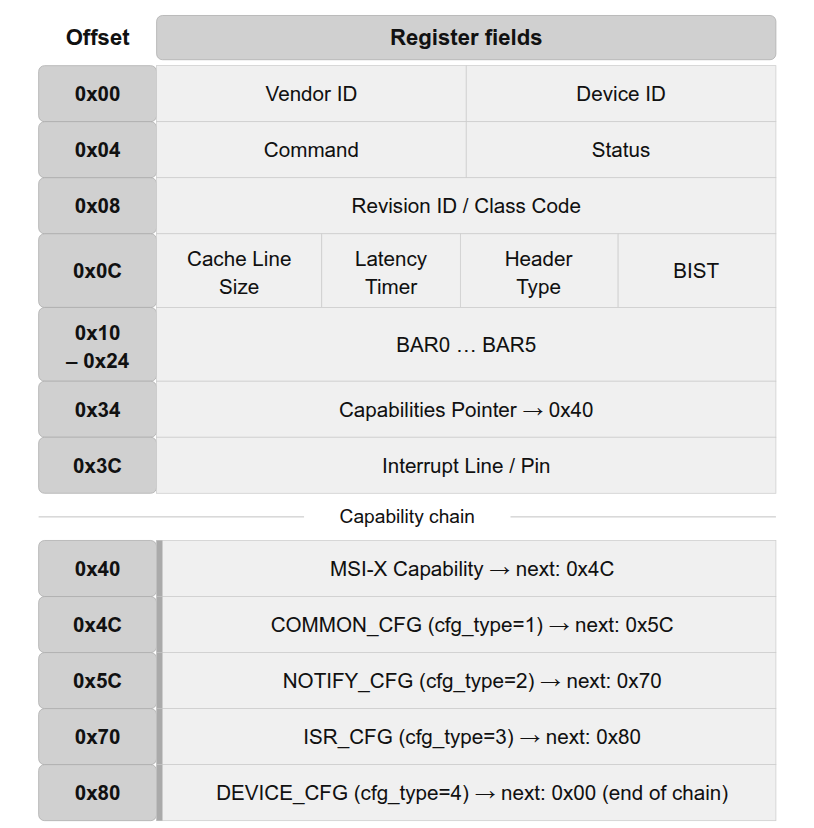
\includegraphics[width=0.8\textwidth]{figures/pci-config-layout.png}
    \caption{Virtual PCI Device Configuration Space Layout}
    \label{fig:pci-config-layout}
\end{figure*}

\subsection{VirtIO Configuration Stage}
\label{sec:virtio-config-stage}

After the first stage is complete, the guest PCI subsystem has allocated MMIO addresses for each BAR. In the second stage, the guest driver accesses the registers of each functional region through MMIO based on the BAR and offset information recorded in the Capabilities, performing the VirtIO handshake with the virtual device. These accesses trigger KVM\_EXIT\_MMIO, which is handled by vmsh's existing MMIO interception mechanism.

The VirtIO handshake follows the state machine defined by the VirtIO specification, with the guest driver triggering state transitions at each stage by writing to the device\_status register in the COMMON\_CFG region. This study implements the following handshake process for the virtual device:

\begin{enumerate}
    \item \textbf{Feature negotiation}: The guest driver reads the device feature bits advertised by the virtual device, selects the features mutually supported by both sides, writes the result to the driver feature bits, and sets the FEATURES\_OK status bit. The virtual device verifies whether the features selected by the driver are valid; if not, it rejects FEATURES\_OK and the driver aborts initialization. After successful negotiation, both sides establish the set of mutually supported features, and the driver proceeds to the virtqueue setup stage.

    \item \textbf{Virtqueue setup}: The virtqueue is a shared memory structure for exchanging I/O requests and responses between the guest driver and the virtual device. The guest driver configures the virtqueue's descriptor table, available ring, and used ring in guest memory, and notifies the virtual device of these memory addresses through COMMON\_CFG registers. The virtual device records these addresses for accessing the virtqueue in guest memory during subsequent I/O processing.

    \item \textbf{DRIVER\_OK}: After completing the above configuration, the guest driver writes the DRIVER\_OK status bit, marking the device as ready. The virtual PCI device implemented in this study activates the device upon receiving DRIVER\_OK, and the device then enters the I/O processing phase.
\end{enumerate}

After the above two initialization stages, the guest has discovered and initialized the virtual device emulated by vmsh through the standard VirtIO-PCI protocol, and subsequent I/O data exchange can proceed on this foundation.

\section{MSI-X Interrupt Injection}
\label{sec:msix-injection}

After the device completes VirtIO-PCI initialization, it enters the I/O processing phase. When the device finishes processing an I/O request issued by the guest, it needs to notify the guest driver via an interrupt to retrieve the result. As described in Section~\ref{sec:arch-overview}, vmsh's existing irqfd interrupt path is unavailable under the Split IRQChip architecture; this study proposes using KVM\_SIGNAL\_MSI to deliver interrupts directly to the LAPIC, without depending on the GSI routing table and IOAPIC, enabling the interrupt mechanism to work under both Full and Split IRQChip architectures. This section describes the specific implementation of this interrupt path.

\subsection{KVM\_SIGNAL\_MSI Interrupt Mechanism}
\label{sec:kvm-signal-msi}

KVM provides the KVM\_SIGNAL\_MSI interface, which allows the caller to deliver an interrupt directly to the target vCPU's LAPIC using an MSI message (address and data) as parameters. The address specifies the target LAPIC's address, and the data contains information such as the interrupt vector.

\begin{sloppypar}
In vmsh's existing interrupt path, the irqfd mechanism depends on the GSI routing table and in-kernel IOAPIC established by the hypervisor during startup: the interrupt signal is routed through the GSI routing table to find the corresponding IOAPIC pin, which then forwards it to the target LAPIC. However, under the Split IRQChip architecture, this infrastructure does not exist within the KVM kernel, rendering vmsh's existing irqfd path inoperable. Although KVM provides the KVM\_SET\_GSI\_ROUTING interface for updating the routing table, and vmsh could architecturally invoke it via ptrace injection, the semantics of this interface is to replace the entire routing table rather than add a single entry, and KVM does not provide an API to read the existing routing table. vmsh cannot know the hypervisor's existing entries for merging; writing blindly would overwrite the hypervisor's routing configuration, causing interrupts for other devices to fail.
\end{sloppypar}

\begin{sloppypar}
In contrast, KVM\_SIGNAL\_MSI writes interrupts directly to the LAPIC, each call is independent, does not require pre-established entries in the GSI routing table, and does not require the existence of an in-kernel IOAPIC. The MSI message itself contains complete interrupt delivery information, and each call only needs the parameters to complete interrupt injection. This study adopts KVM\_SIGNAL\_MSI as the interrupt injection method used by PCI transport, leveraging its independence from interrupt routing infrastructure to enable vmsh to deliver interrupts to the guest even in environments where the irqfd path is unavailable.
\end{sloppypar}

When using KVM\_SIGNAL\_MSI, the caller needs to provide the address and data of the MSI message as parameters. In a standard VirtIO-PCI device, the guest driver writes the address and data of the interrupt vector to the device's MSI-X Table during initialization; vmsh needs to intercept these writes and maintain the corresponding interrupt vector parameters for use during subsequent interrupt injection.

\subsection{MSI-X Table and Interrupt Vector Management}
\label{sec:msix-table}

The MSI-X Table is a structure used by PCI devices to store interrupt vectors, located within the memory region mapped by the device's BAR. Each table entry records the address and data of one interrupt vector; the guest driver writes interrupt vectors to this table via MMIO during device initialization, informing the device which target LAPIC to deliver interrupts to and which vector to use.

For vmsh, the MSI-X Table is the source for obtaining interrupt vector parameters. This study maps the MSI-X Table region to BAR4 of the PCI virtual device. When the guest driver writes address and data values via MMIO, a KVM\_EXIT\_MMIO is triggered; vmsh intercepts it and records the address and data into the MSI-X Table structure maintained internally by the virtual device. When the device subsequently needs to send an interrupt, vmsh retrieves the corresponding interrupt vector parameters from this structure and uses them as input parameters for KVM\_SIGNAL\_MSI to deliver the interrupt to the guest through KVM.

\subsection{Interrupt Injection Implementation}
\label{sec:injection-impl}

KVM\_SIGNAL\_MSI is a KVM ioctl and therefore needs to be invoked through the VM file descriptor (vm\_fd). However, vm\_fd is obtained from KVM by the hypervisor when creating the VM; vmsh, as an external process, does not hold this file descriptor and therefore cannot directly invoke KVM\_SIGNAL\_MSI.

\begin{sloppypar}
Therefore, this study utilizes vmsh's existing ptrace syscall injection mechanism to inject the ioctl call into a hypervisor vCPU thread that has been suspended by ptrace, borrowing the vm\_fd held by the hypervisor to execute KVM\_SIGNAL\_MSI. The specific procedure is as follows: vmsh first assembles the address and data recorded in the MSI-X Table into a kvm\_msi structure and writes it to the hypervisor's address space; it then saves the thread's registers and the original instruction at the instruction pointer location, writes a syscall instruction at the instruction pointer position, and sets the registers to the ioctl parameters (vm\_fd, KVM\_SIGNAL\_MSI, address of the kvm\_msi structure); vmsh then advances thread execution via ptrace, causing the kernel to execute the ioctl and complete the interrupt injection; finally, it restores the original instruction and registers, returning the hypervisor thread to its pre-injection state.
\end{sloppypar}

The ptrace syscall injection method described above is the preliminary implementation adopted by this study for interrupt triggering. As part of the PCI transport synchronous I/O model, this approach is implemented in a simpler synchronous manner to verify whether the interrupt path of PCI transport can operate correctly.

Figure~\ref{fig:io-roundtrip} shows a complete I/O round-trip after the device is ready. (1) The guest driver writes to NOTIFY\_CFG to initiate an I/O request, triggering KVM\_EXIT\_MMIO. (2) vmsh intercepts it via ptrace, reads the virtqueue, and executes disk I/O. (3) Upon completion, vmsh retrieves the interrupt vector parameters from the MSI-X Table and injects KVM\_SIGNAL\_MSI into the hypervisor vCPU thread via ptrace syscall injection; KVM writes the interrupt to the LAPIC. (4) vmsh then restores the thread state and resumes the vCPU. (5) Upon VM entry, the vCPU delivers the pending interrupt, and the guest retrieves the I/O result after receiving the interrupt.

\begin{figure*}[htbp]
    \centering
    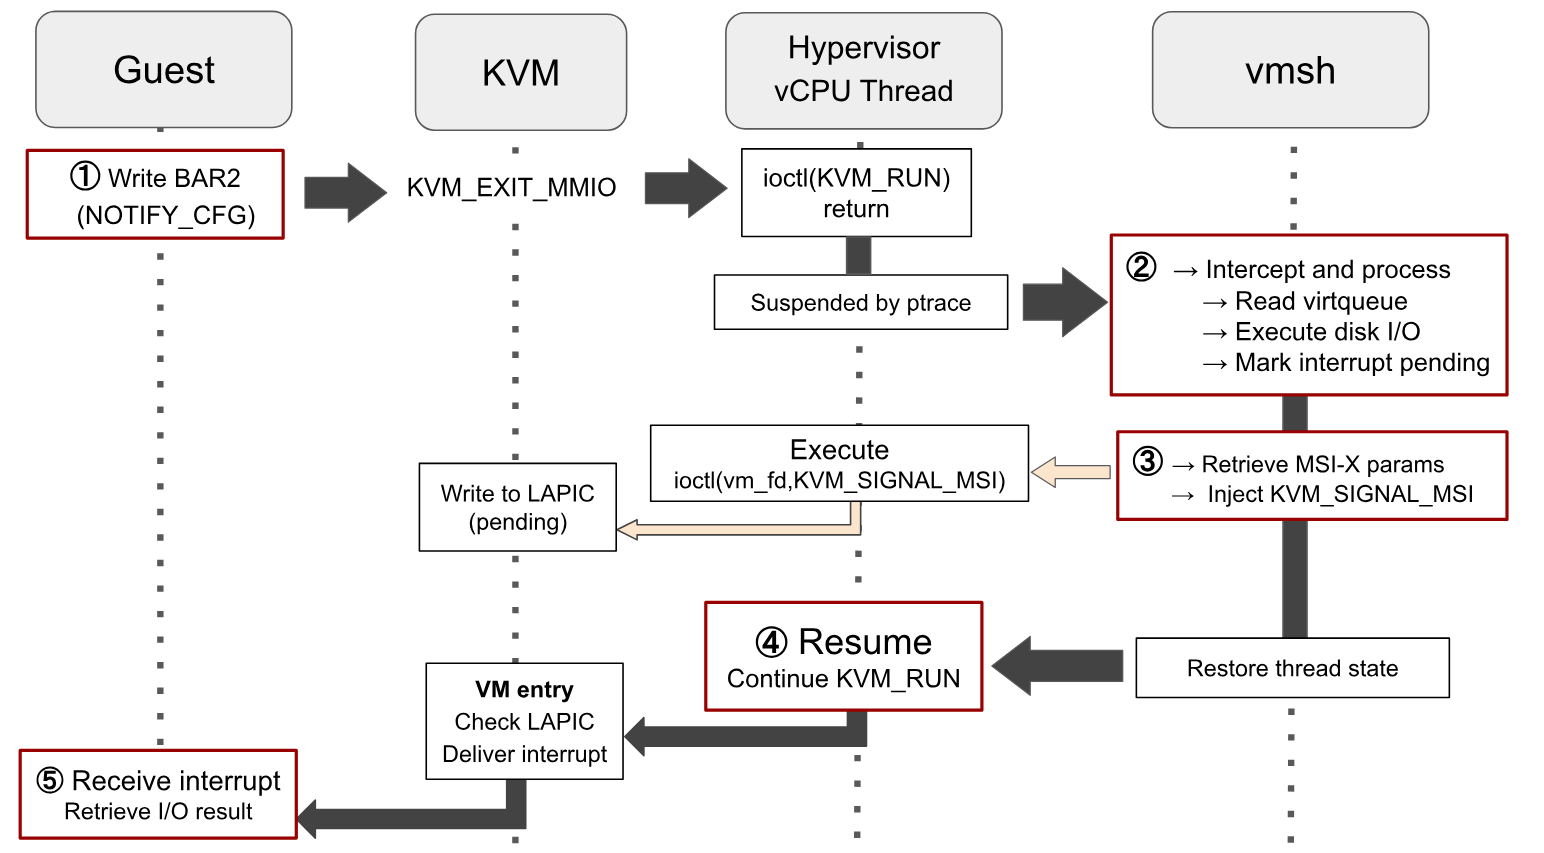
\includegraphics[width=1.0\textwidth]{figures/io-roundtrip.png}
    \caption{A Complete I/O Round-Trip}
    \label{fig:io-roundtrip}
\end{figure*}

This study integrates the mechanisms from Section~\ref{sec:pci-rescan} through Section~\ref{sec:msix-injection} using the synchronous I/O model described above, covering device discovery, Port I/O interception, PCI device emulation, and MSI-X interrupt injection, to implement a complete data path from the guest issuing an I/O request to receiving an interrupt response, verifying the feasibility of the non-cooperative PCI device emulation scheme.

\end{ZhChapter}

% 章節四 Chapter 4
\begin{ZhChapter}

\chapter{Experiment and Result}

\section{Functional Validation and Generality}

\subsection{PCI Device Discovery and Initialization}

\begin{figure*}[htbp]
    \centering
    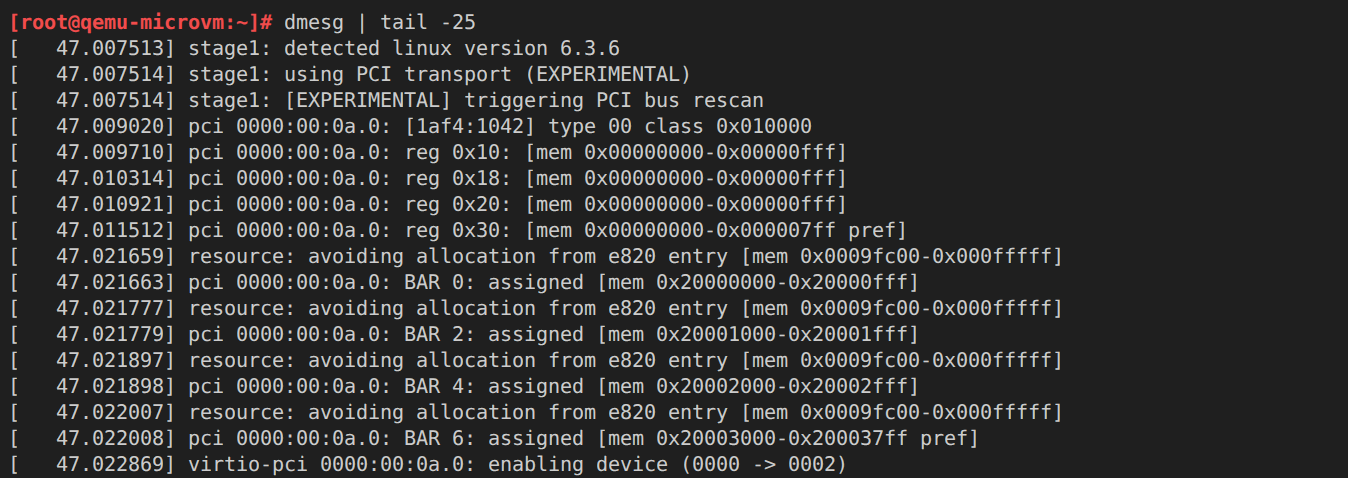
\includegraphics[width=1.0\textwidth]{figures/dmesg-pci-discovery.png}
    \caption{dmesg log of PCI device discovery and BAR assignment (QEMU)}
    \label{fig:dmesg-pci-discovery}
\end{figure*}

\begin{figure*}[htbp]
    \centering
    
\includegraphics[width=1.0\textwidth]{figures/dmesg-virtio-negotiation.png}
    \caption{dmesg log of VirtIO negotiation completion (QEMU)}
    \label{fig:dmesg-virtio-negotiation}
\end{figure*}

\begin{figure*}[htbp]
    \centering
    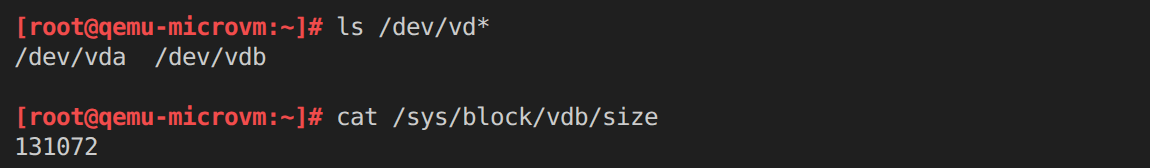
\includegraphics[width=1.0\textwidth]{figures/guest-vdb-query.png}
    \caption{Guest userspace query of the vdb device}
    \label{fig:guest-vdb-query}
\end{figure*}

\subsection{Block I/O and Filesystem Validation}

\begin{figure*}[htbp]
    \centering
    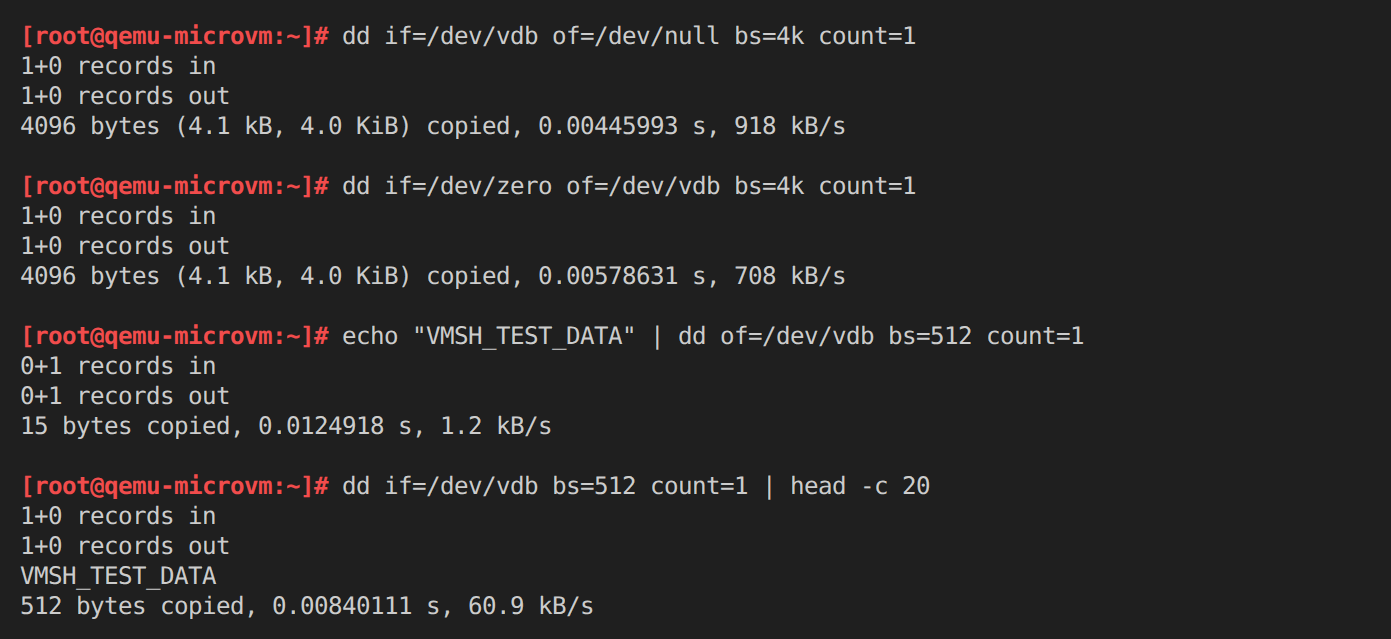
\includegraphics[width=1.0\textwidth]{figures/block-io-test.png}
    \caption{Block I/O read/write and data integrity test (QEMU)}
    \label{fig:block-io-test}
\end{figure*}

\begin{figure*}[htbp]
    \centering
    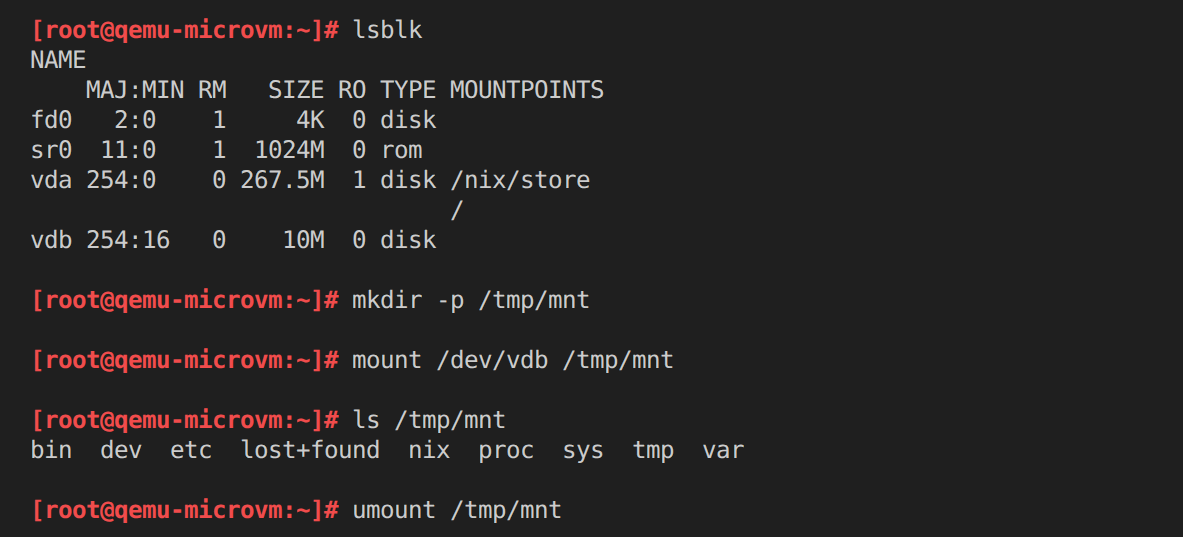
\includegraphics[width=1.0\textwidth]{figures/ext4-mount-test.png}
    \caption{ext4 filesystem mount test (QEMU)}
    \label{fig:ext4-mount-test}
\end{figure*}

\subsection{Cloud Hypervisor Validation}

\begin{figure*}[htbp]
    \centering
    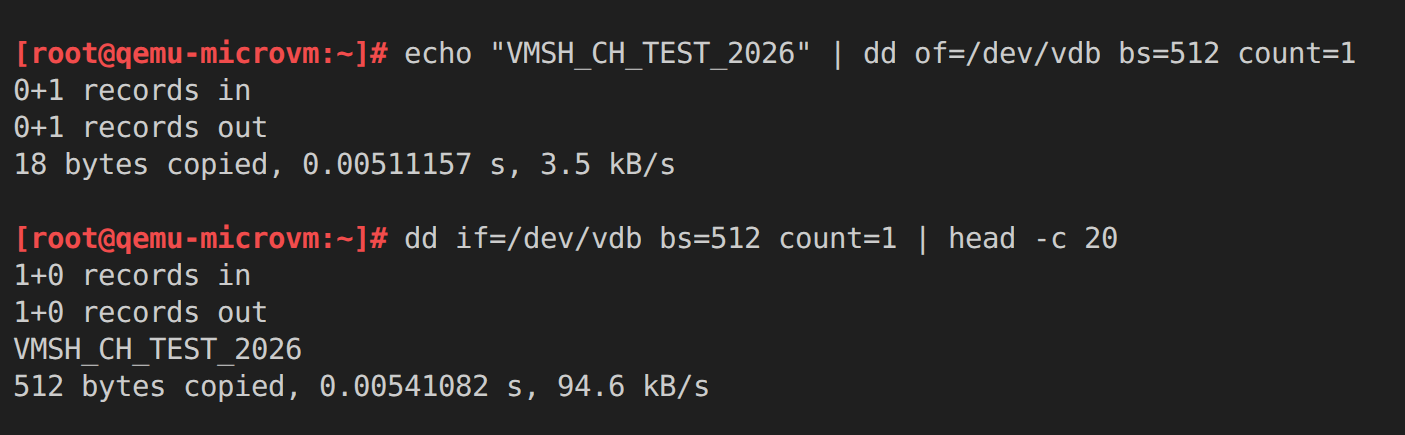
\includegraphics[width=1.0\textwidth]{figures/ch-data-integrity.png}
    \caption{Data integrity test (Cloud Hypervisor)}
    \label{fig:ch-data-integrity}
\end{figure*}

\begin{figure*}[htbp]
    \centering
    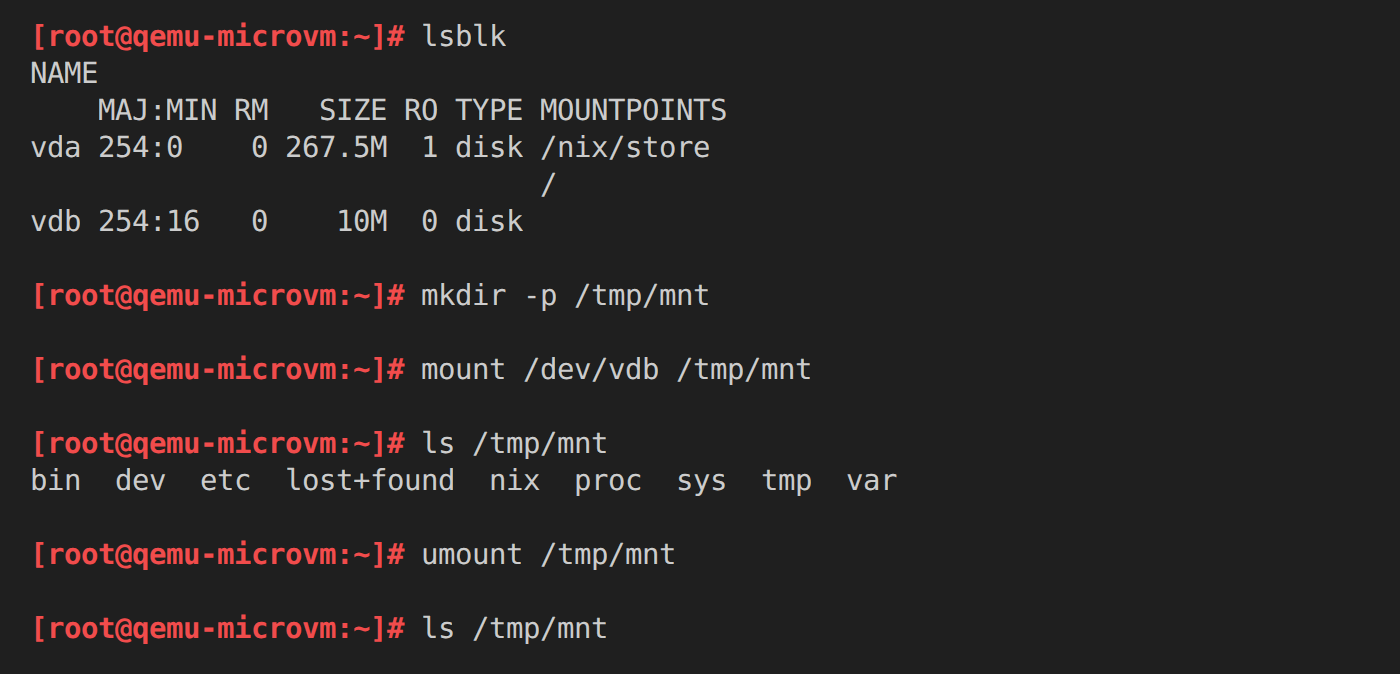
\includegraphics[width=1.0\textwidth]{figures/ch-ext4-mount.png}
    \caption{ext4 filesystem mount test (Cloud Hypervisor)}
    \label{fig:ch-ext4-mount}
\end{figure*}

\end{ZhChapter}

% 章節五 Chapter 5
\begin{ZhChapter}

\chapter{Conclusion and Future Work}
\label{ch:conclusion}

\section{Conclusion}
\label{sec:conclusion}

This study extends the functionality of vmsh by implementing VirtIO over PCI transport while maintaining the non-cooperative and hypervisor-agnostic design philosophy, enabling vmsh to successfully support Cloud Hypervisor. The main contributions are as follows:

\begin{enumerate}
    \item \textbf{PCI device emulation in a non-cooperative environment.} As an external process independent of the hypervisor, vmsh must complete device emulation from the outside without hypervisor cooperation. This study extends vmsh's side-load library mechanism to trigger PCI rescan in the guest, and intercepts Port I/O instructions issued by the guest (KVM\_EXIT\_IO) via ptrace, responding to the guest's accesses to the virtual device's PCI Configuration Space so that the guest can discover the PCI virtual device emulated by vmsh during the rescan process. On this basis, a complete VirtIO-PCI device emulation is implemented, including PCI Configuration Space, BAR mapping, and virtqueue configuration, enabling the guest's virtio-pci driver to complete initialization and perform block I/O.

    \item \textbf{Resolving interrupt mechanism compatibility issues to expand vmsh's hypervisor support.} vmsh's existing interrupt injection mechanism (irqfd) relies on the Full IRQChip architecture, limiting vmsh to operate only under hypervisors that adopt this architecture (e.g., QEMU). This study adopts KVM\_SIGNAL\_MSI to implement MSI-X interrupt injection, which does not depend on a specific IRQChip architecture, enabling vmsh to also support hypervisors that adopt Split IRQChip (e.g., Cloud Hypervisor).

    \item \textbf{Cross-hypervisor validation confirming correctness and generality.} This study performs validation in both QEMU (Full IRQChip) and Cloud Hypervisor (Split IRQChip) environments. Functional validation covers PCI device discovery, initialization, interrupt path establishment, and block I/O, all of which pass in both environments. Additionally, correctness testing with xfstests shows that this study's PCI transport prototype implementation, under a 1 vCPU configuration, fails on the same test cases as vmsh's existing MMIO transport, providing preliminary reference data for the correctness of the PCI transport mechanism.
\end{enumerate}

\section{Future Work}
\label{sec:future-work}

This study validated the feasibility of non-cooperative PCI transport using a synchronous I/O model. Future development can proceed in the following directions:

\begin{enumerate}
    \item \begin{sloppypar}\textbf{Asynchronous I/O model.} This study's prototype implementation adopts a synchronous I/O model where each I/O operation blocks the vCPU thread, limiting operation to a 1 vCPU configuration only. Future work can refer to the asynchronous architecture of vmsh's existing MMIO implementation, receiving guest I/O requests via ioeventfd, processing them asynchronously on a dedicated thread, and injecting interrupts via KVM\_SIGNAL\_MSI upon completion, enabling the PCI transport to achieve xfstests validation results comparable to vmsh's existing implementation in a multi-vCPU environment.\end{sloppypar}

    \item \textbf{Performance testing.} After completing the asynchronous I/O model, performance testing can be conducted following the methodology used in the original vmsh paper, comparing against vmsh's existing MMIO transport and QEMU's native virtio-blk device to evaluate the performance of PCI transport.

    \item \textbf{Integration with vmsh's existing features.} This study has validated the feasibility of attaching a block device via PCI transport. vmsh's complete workflow includes, in addition to the block device, a Stage2 environment for establishing isolated containers inside the guest and a console interface for interactive terminal access. Future work can integrate PCI transport with these features, enabling vmsh to provide the same complete functionality on Cloud Hypervisor as the existing MMIO transport.
\end{enumerate}

\end{ZhChapter}

% 新增你自己的章節... Add chapters here

% 參考文獻，請在段落上隨意註解，你同時需要 reference.bib
\addcontentsline{toc}{chapter}{References}
\renewcommand{\bibname}{References}
\begin{sloppypar}
\printbibliography
\end{sloppypar}


\end{document}
